% ====================================================================
%+
% SECTION:
%    MW_Astrometry.tex
%
% CHAPTER:
%    galaxy.tex
%
% ELEVATOR PITCH:
%
%-
% ====================================================================

\section{Astrometry with LSST: Positions, Proper Motions, and Parallax}
\def\secname{MW_Astrometry}\label{sec:\secname}

\credit{dgmonet}, \credit{DanaCD}, \credit{jgizis}, \credit{mliu},
\credit{caprastro}, \credit{willclarkson}, \credit{yoachim}

A number of Milky Way science cases of interest to the Astronomical
community will depend critically on the astrometric accuracy LSST will
deliver. While ``astrometry'' is not a science case in the framework
of this white paper, LSST's astrometric performance will be sensitive
to the particular choice of observing strategy.
%While astrometry is not a science case, high astrometric accuracy enables
%a large number of science cases.
Hence, the LSST Observing Strategy needs to be examined for systematic
trends that might mitigate or even preclude precise measures of
stellar positions, proper motions, parallaxes, and perturbations that
arise from unseen companions.

\autoref{sec:\secname:MW_Astrometry_measurements} highlights two
science cases at opposite scales of distance from the Sun that require
accurate and precise astrometry and/or proper motion
measurements. \autoref{sec:\secname:MW_Astrometry_metrics} develops
Metrics for LSST's astrometric performance, and discusses Figures of
Merit for the two highlighted science cases. These metrics are applied to two example OpSim runs in
\autoref{sec:\secname:MW_Astrometry_OpSim}. Finally in Section
\ref{sec:\secname:MW_Astrometry_furtherwork}, the work that is still
needed is discussed, both in terms of the Metrics and the Figures of
Merit that depend on them.

%Each of these cases stresses different aspects of the LSST hardware, software,and observing strategies.

%, here we highlight three representative science cases.
%that illustrate the various impacts of the observing strategy might
%be:
%To highlight the
%various astrometric impacts of the strategy, three science cases have
%been chosen for particular attention:

%\subsection{Introduction: Astrometry as a special case}
%\label{sec:\secname:MW_Astrometry_intro}

\subsection{Target Measurements and Discoveries}
\label{sec:\secname:MW_Astrometry_measurements}

\begin{itemize}
\item[1.] Identification of Streams in the Galactic Halo using proper motions.
\item[2.] A complete sample of stars in the solar neighborhood.
\end{itemize}
%\item The tie between the Radio and Optical realizations of the International Celestial Reference System.
%\item The specific and ensemble agreement between LSST and Gaia parallaxes.

{\bf 1. Streams in the Galactic halo}

Much of the Milky Way's stellar halo was built by the accretion of smaller galaxies. Given that these galaxies
were generally of low mass, their tidal debris should still form coherent structures in phase space, especially
in the outer Galaxy where dynamical times are long. The identification of these streams would allow
a reconstruction of the accretion history of the Milky Way. Tides also lead to the dissolution of globular clusters,
leaving notably thin streams that serve as sensitive tracers both of the Galactic potential and of the presence of dark
subhalos.

A relatively small number of streams, originating from both dwarfs and globular clusters, have been identified via photometry
of individual stars in large surveys such as SDSS\@. However, only the highest surface brightness structures can be found
in this manner, and it is often difficult to trace the streams over their full extent. LSST will enable streams to be identified
by stellar proper motions, and combined with targeted follow-up spectroscopy, will yield full 6-D position and velocity measurements suitable for dynamical modeling.
Further, it will allow the discovery of tidal debris that is no longer spatially coherent but which can be unambiguously identified in phase space.

Finally, streams and other kinematically-distinct halo substructure
can be identified and characterized by combining proper motions and
photometry in reduced proper-motion diagrams \citep[e.g.,][]{carlin12},
and by analyzing proper-motions of tracers such as
RR Lyrae and giants over large portions of the sky \citep[e.g.,][]{casettidinescu15}.

{\it Response to observing strategy:} Most stars in streams will be main-sequence stars, and the old main sequence turnoff  is located at $r\sim24$ at a distance of 100 kpc.
The nominal LSST proper motion precision at this magnitude is 1 mas yr$^{-1}$, corresponding to about 475 km s$^{-1}$ at this distance. The proper motion
measurements will be better for brighter stars, but in general ensembles of stars will be necessary for accurate measurements. To make accurate proper motion measurements for faint stars, several key components are required. First, a zero point must be established, possibly via background galaxies located in each field. Next, the observations must cover a sufficient range of epochs to reliably detect linear proper motions.

To identify streams over their full lengths of many degrees of the sky, relative astrometry over small fields will not be sufficient. Therefore the absolute astrometric frame is important. Matching the optical astrometry to the radio International Celestial Reference System (ICRS) relies on measuring accurate positions for objects visible in both wavelength regimes.
These are typically distant QSOs. Unfortunately, many QSOs have detectable optical or radio structures that degrade the positions or suggests a displacement between the location of the sources of the radio and optical radiation. LSST will need to identify a large number of point-like QSOs based on their colors and variability.

Since the number of galaxies is overwhelming toward faint magnitudes,
these must be exploited to produce a reliable absolute
proper-motion zero point. By using Gaia stars at the bright end
as absolute proper-motion calibrators we can quantify the precision
and accuracy of background galaxies as a secondary link to an inertial reference system, and thus improve the calibration at the faint end of the survey.

%The tie between the radio and optical reference frames relies on measuring accurate positions for objects visible in both wavelength regimes.  Whereas there are optical variable stars with radio emission, most have associated optical nebulosity that degrades the accuracy of the optical positions. The typical radio+optical object is a QSO.  Unfortunately, many QSOs have detectable optical or radio structures that degrade the positions or suggests a displacement between the location of the sources of the radio and optical radiation.  The major contribution from LSST will be the identification of a large number of QSOs based on their colors that have minimal (if any) spatially extended structure.  The impact of this search has no obvious impact on the cadence other than temporal coverage to identify variability.

{\bf 2. A complete sample of stars in the solar neighborhood}

The direct solar neighborhood offers our only chance to get make a complete sample of stars, brown dwarfs, and stellar remnants that encompass the entire formation and dynamical history of the Milky Way. While Gaia will offer parallax measurements for perhaps billions of stars, its faint magnitude limit of $G\sim 20$ will limit its measurements of the lowest-mass objects
and remnants to nearby objects, much less than the thin disk scale height of $\sim 300$ pc. For example, Gaia can only measure parallaxes for $0.2 M_{\odot}$ M dwarfs to about 100 pc
and $0.1 M_{\odot}$ M dwarfs to only \emph{10 pc}, showing that Gaia is ill-suited for studies of the coolest dwarfs. By contrast, LSST can measure parallaxes for $> 10^5$ M dwarfs and thousands of L/T brown dwarfs (the coolest Y dwarfs are too faint even for LSST; little contribution is likely here beyond the sample provided by WISE). Gaia will likewise be limited to cool white dwarfs within $\sim 100$ pc with which to estimate the age of the disk, and the thick disk and halo will be out of reach. LSST can directly compare white dwarf luminosity functions to determine precise differential ages for the thin disk, thick disk, and halo.

{\it Response to observing strategy:} Successfully completing this project will require parallax measurements much fainter than possible with Gaia as well as a verification that the LSST and Gaia parallax measurements are consistent in the overlapping magnitude range.

The measurement of stellar parallax puts the substantial constraints on the observing cadence. There are two major issues: the need to sample a wide range of parallax factor (related to time of year), and breaking the correlation between differential color refraction and parallax factor.

``Parallax factors" characterize the ellipse of the star's apparent motion as seen over the course of a year. The shape of the ellipse is given by the Earth's orbit and is not a free parameter in the astrometric solution. The amplitude of the right ascension parallax factor is close to unity while the amplitude of the declination parallax factor is dominated by the sine of ecliptic latitude.
The right ascension parallax factor has maximum amplitude when the star is approximately six hours from the Sun, so the optimum time for parallax observing is when the
star is on the meridian near evening or morning twilight. Atmospheric refraction displaces the star's apparent position in the direction of the zenith by an amount dependent on both the wavelength of the light and the distance to the zenith. Whereas the measured position of star is a function of the total refraction, the measurement of parallax
and proper motion depends on the differences in the refraction as a function of the color of each star and the circumstances of the observations.  This
dependence is called differential color refraction. The combination of parallax factor and differential color refraction leads to two rules:
\begin{itemize}
\item [1] Observations need to cover the widest possible range in parallax
factor.
\item [2] The correlation between parallax factor and hour angle in the observations needs to be minimized.
\end{itemize}

%with respect to the meanmotion of the reference frame.

%The search for faint proper motion stars has two key components.  The first is the need to identify stars that move from the ensemble of other image features that can cause confusion.  For example, a compact group of stars that contains one or more stars of variable brightness can confuse the catalog correlation algorithm.  The other is the need to establish the zero point. For the case of relative astrometry, meaning the measurement of relative positions in an image, the question remains on how to remove the mean motion of the reference frame.  For example, astrometry on certain classes of galaxies might produce a zero point of sufficient accuracy.  This leads to a third constraint on the observing cadence.
% \begin{itemize}
%\item [3)] Observations must cover a sufficient range of epochs so that stars with
%linear or periodic motions can be identified at a high level of confidence.
%\end{itemize}


%\subsection{Sensitivity of parallax measurements to observing strategy}
%\label{sec:\secname:MW_Astrometry_cadence}

%\medskip


\subsection{Metrics and Figures of Merit for LSST's delivered astrometric accuracy}
\label{sec:\secname:MW_Astrometry_metrics}

%\medskip

First we discuss metrics for the observing strategy that affect all of
LSST's astrometric measurements, then discuss figures of merit for the
two science cases. (The three general metrics were identified years ago and
are already in the suite of MAF utilities, but they should be reviewed
prior to making final decisions.)

\begin{itemize}
\item[A)] For each LSST field, the parallax factors at each epoch of
observation need to be computed.  The ensemble of these must be checked for
sufficient coverage of the parallactic ellipse.  In particular, the number of
measures with RA parallax factor less than --0.5 and greater than +0.5
needs to be tallied because these carry the most weight in the solution
for the amplitude (parallax).
\item[B)] For each LSST field, the hour angle of the observation needs to be
computed, and the correlation between hour angle and parallax factor
needs to be examined for significance.  The observing strategy must minimize
the number of fields with this correlation.
\item[C)] The epochs of observation for each field must be checked for a
reasonable coverage over the duration of the survey and to avoid
collections of too many visits during a few short intervals.
\end{itemize}

For the stream project discussed above, a simple to state (but perhaps complex to implement) figure of merit
is the number of streams that can be discovered in LSST via their proper motions. As a first
attempt, it would be reasonable to assume about 100 halo streams from old, metal-poor dwarf galaxies with
stellar masses $10^5-10^7 M_{\odot}$ distributed as $r^{-3.5}$. The stream widths and internal velocity
dispersions can be set from galaxy scaling relations, and their 3-D velocities consistent with a simple Galactic mass
model at their radii. Setting the stream lengths is more complicated, but should cover a large range from a few to many kpc.
Over a given area, the stream ``S/N" can roughly be taken as the number of stream stars (identified via proper motion, color, and magnitude)
divided by the square root of the number of field stars. For globular clusters, a similar number of streams could be included, but these should have much smaller widths (10s of pc)
and typical masses $10^4-10^5 M_{\odot}$. Eventually it would be desirable to use actual simulated stream parameters taken from cosmological models of the Milky Way (e.g.,
from the Aquarius simulation).

Solar neighborhood projects will be sensitive to the general parallax and proper motion metrics discussed above. More specific science figures of merit are {\it required} at this stage.  For example, the precision of the differential age measurement between the thin disk and halo, which would depend on the number of white dwarfs that can be isolated
from each population.

\subsection{OpSim Analysis}
\label{sec:\secname:MW_Astrometry_OpSim}

Here we present initial analysis of LSST's astrometric
performance. Two example strategies are assessed: the current (as of
December 2015) baseline strategy, \opsimdbref{db:baseCadence}, and the
PanSTARRS-like cadence, \opsimdbref{db:opstwoPS}, which greater
spatial uniformity and superior coverage of the Galactic Plane.

\subsubsection{Metrics: Parallax and proper motion precision}

Here we present the expected astrometric performance of LSST as a function of
location on-sky, subdivided by elapsed time in the survey
(Figures~\ref{fig_astrom_ByTime_PACoverage} -
\ref{fig_astrom_ByTime_paError}), and for three extreme choices of filters in
which an object is detected (Figures~\ref{fig_astrom_ByFilter_PACoverage} -
\ref{fig_astrom_ByFilter_paError}).  Astrometric performance for parallax is
quantified using the following metrics:
\begin{itemize}
  \item[1.] Parallax factor coverage (following metric A of \autoref{sec:\secname:MW_Astrometry_metrics}); values farther from 0 are better). See Figures \ref{fig_astrom_ByTime_PACoverage} \&  \ref{fig_astrom_ByFilter_PACoverage};
    \item[2.] Parallax-Hour angle correlation (metric B of \autoref{sec:\secname:MW_Astrometry_metrics}; values closer to 0 are better). See Figures \ref{fig_astrom_ByTime_PADegen} \& \ref{fig_astrom_ByFilter_PADegen};
      \item[3.] Proper motion error, for a star at apparent magnitude 21.0 in the filter specified (this addresses the distribution of measurement epochs, as recommended in Metric C in \autoref{sec:\secname:MW_Astrometry_metrics}; smaller values are better). See Figures \ref{fig_astrom_ByTime_pmError} \& \ref{fig_astrom_ByFilter_pmError};
        \item[4.] Parallax error, for a star at apparent magnitude 21.0 in the filter specified (smaller values are better). See Figures \ref{fig_astrom_ByTime_paError} \& \ref{fig_astrom_ByFilter_paError}.
\end{itemize}

{\it Limitations of this presentation:}
\begin{itemize}
  \item[i.] The spatial maps are clipped at $95\%$~in order to keep
    the color-scale at a sensible range; in some cases this has had
    the side effect of removing parts of the spatial coverage in the
    \opsimdbref{db:baseCadence} maps.

  \item[ii.] No attempt has been made in this subsection to account
    for spatial confusion in high-density regions. While this
    confusion would be the same whatever observing strategy was
    chosen, the numbers for proper motion and parallax uncertainty
    should be regarded as lower limits.

    \item[iii.] The choice of fiducial apparent magnitude $r = u = y =
      21.0$~is not terribly well-motivated in this subsection. It
      would be informative to repeat the analysis for a range of
      target apparent magnitudes that are better-matched to the
      specific science cases.

      \item[iv.] The comparison between single-filter and $ugrizy$
        detections likely overestimates the measurement precision for
        the $u$-only and $y$-only detections, as an object only
        detected in a single filter may well not be detected in all
        images taken in that filter. While the comparison between
        filter subsets for a given strategy may therefore be highly
        approximate, the comparison between strategies for the same
        filter should be more reliable.

  \item[v.] We have not yet subdivided the samples by a meaningful
    spatial co-ordinate (galactic latitude would be the obvious
    choice). A large part of the breadth of the various metric values in
    \opsimdbref{db:baseCadence} as compared to \opsimdbref{db:opstwoPS} may be
      due to spatial nonuniformity of the sampling; replotting the
      histograms coded by galactic latitude would be highly informative in this context.

\end{itemize}

{\it Indications at this date:} Despite these limitations, we note the following:

\begin{itemize}
  \item[I1.] Taking snapshots of the survey at various stages of completion (Figures \ref{fig_astrom_ByTime_PACoverage} -  \ref{fig_astrom_ByTime_paError}), the PanSTARRS-like cadence is no worse than \opsimdbref{db:baseCadence}, and by most measures offers better performance;
\item[I2.] As might be expected, the distribution of metric values for the PanSTARRS-like cadence is narrower than for \opsimdbref{db:baseCadence} - thus astrometric survey uniformity is improved;
\item[I3.] For the extremes of object color (objects detected only in the bluest or only in the reddest filter), the differences between strategies is weaker. The run \opsimdbref{db:baseCadence} still shows a population with poorer parallax measures (although this might be due to coverage of regions simply not covered at all by the PanSTARRS-like strategy).
\end{itemize}

%% In the current incarnation, these will be big figures on the page. Consider
%% finding a way to summarize them!
\begin{figure}[ht]
  \begin{center}
  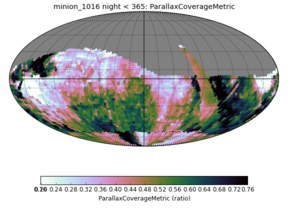
\includegraphics[width=2.0in]{./figs/milkyway/astromPanels/MW_Astrom_paCovge_Baseline_01y_map.png}
  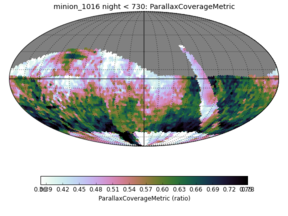
\includegraphics[width=2.0in]{./figs/milkyway/astromPanels/MW_Astrom_paCovge_Baseline_02y_map.png}
  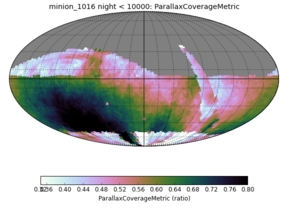
\includegraphics[width=2.0in]{./figs/milkyway/astromPanels/MW_Astrom_paCovge_Baseline_10y_map.png}
  \end{center}
  \begin{center}
  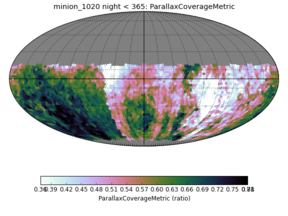
\includegraphics[width=2.0in]{./figs/milkyway/astromPanels/MW_Astrom_paCovge_PanSTARRS_01y_map.png}
  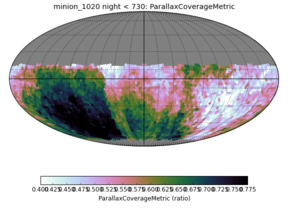
\includegraphics[width=2.0in]{./figs/milkyway/astromPanels/MW_Astrom_paCovge_PanSTARRS_02y_map.png}
  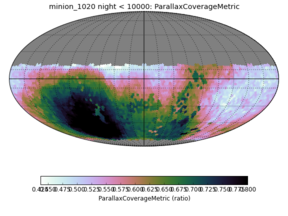
\includegraphics[width=2.0in]{./figs/milkyway/astromPanels/MW_Astrom_paCovge_PanSTARRS_10y_map.png}
  \end{center}

  \begin{center}
  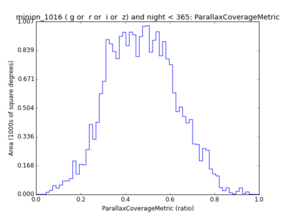
\includegraphics[width=2.0in]{./figs/milkyway/astromPanels/MW_Astrom_paCovge_Baseline_01y_hst.png}
  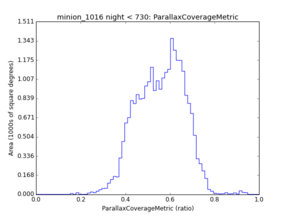
\includegraphics[width=2.0in]{./figs/milkyway/astromPanels/MW_Astrom_paCovge_Baseline_02y_hst.png}
  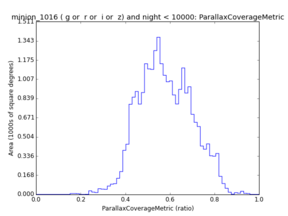
\includegraphics[width=2.0in]{./figs/milkyway/astromPanels/MW_Astrom_paCovge_Baseline_10y_hst.png}
  \end{center}
  \begin{center}
  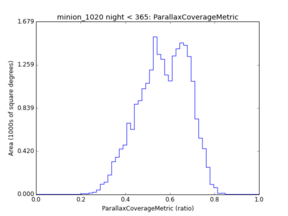
\includegraphics[width=2.0in]{./figs/milkyway/astromPanels/MW_Astrom_paCovge_PanSTARRS_01y_hst.png}
  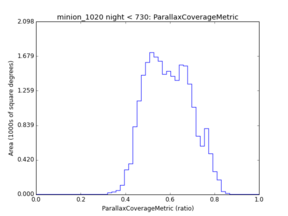
\includegraphics[width=2.0in]{./figs/milkyway/astromPanels/MW_Astrom_paCovge_PanSTARRS_02y_hst.png}
  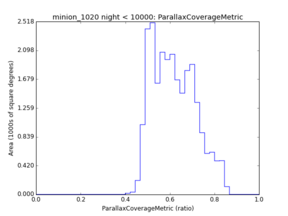
\includegraphics[width=2.0in]{./figs/milkyway/astromPanels/MW_Astrom_paCovge_PanSTARRS_10y_hst.png}
  \end{center}
  \caption{Parallax coverage achieved at different epochs within the survey. {\it Top and Third row:} OpSim run \opsimdbref{db:baseCadence}. {\it Second and bottom row:} OpSim run \opsimdbref{db:opstwoPS} (PanSTARRS-like cadence). Reading left-right, columns represent: {\it Left column:} all observations within the first 365 days of operation; {\it Middle column:} first two years; {\it right column:} the full 10-year survey. Spatial maps are clipped at 95\%, with histogram horizontal scale set to $\pm 1.0$~for easy comparison.}
  \label{fig_astrom_ByTime_PACoverage}
\end{figure}

\begin{figure}[ht]
  \begin{center}
  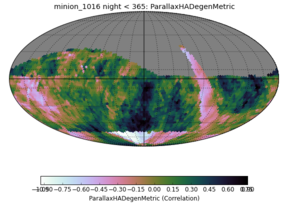
\includegraphics[width=2.0in]{./figs/milkyway/astromPanels/MW_Astrom_paDegen_Baseline_01y_map.png}
  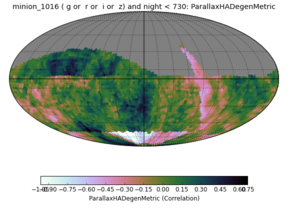
\includegraphics[width=2.0in]{./figs/milkyway/astromPanels/MW_Astrom_paDegen_Baseline_02y_map.png}
  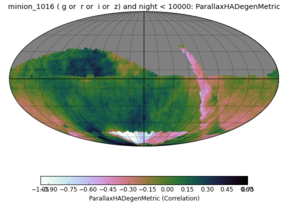
\includegraphics[width=2.0in]{./figs/milkyway/astromPanels/MW_Astrom_paDegen_Baseline_10y_map.png}
  \end{center}
  \begin{center}
  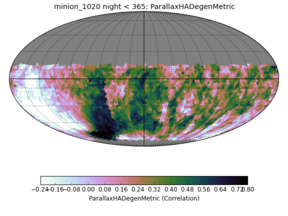
\includegraphics[width=2.0in]{./figs/milkyway/astromPanels/MW_Astrom_paDegen_PanSTARRS_01y_map.png}
  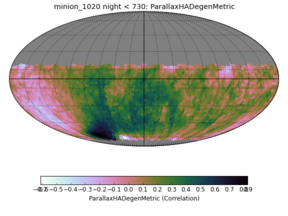
\includegraphics[width=2.0in]{./figs/milkyway/astromPanels/MW_Astrom_paDegen_PanSTARRS_02y_map.png}
  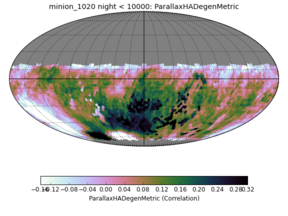
\includegraphics[width=2.0in]{./figs/milkyway/astromPanels/MW_Astrom_paDegen_PanSTARRS_10y_map.png}
  \end{center}

  \begin{center}
  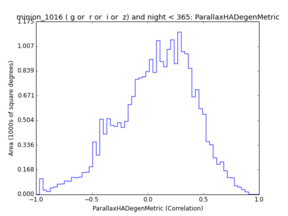
\includegraphics[width=2.0in]{./figs/milkyway/astromPanels/MW_Astrom_paDegen_Baseline_01y_hst.png}
  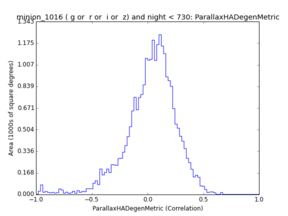
\includegraphics[width=2.0in]{./figs/milkyway/astromPanels/MW_Astrom_paDegen_Baseline_02y_hst.png}
  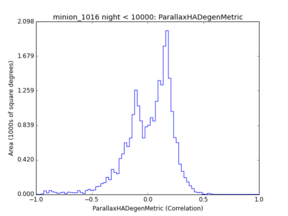
\includegraphics[width=2.0in]{./figs/milkyway/astromPanels/MW_Astrom_paDegen_Baseline_10y_hst.png}
  \end{center}
  \begin{center}
  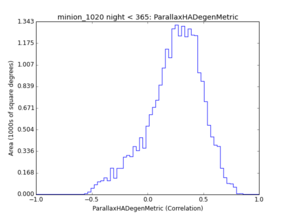
\includegraphics[width=2.0in]{./figs/milkyway/astromPanels/MW_Astrom_paDegen_PanSTARRS_01y_hst.png}
  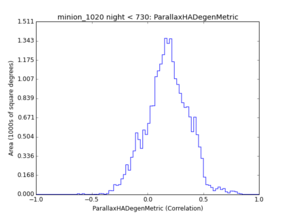
\includegraphics[width=2.0in]{./figs/milkyway/astromPanels/MW_Astrom_paDegen_PanSTARRS_02y_hst.png}
  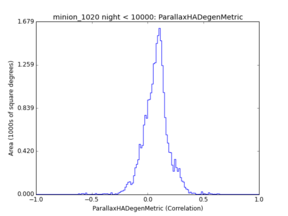
\includegraphics[width=2.0in]{./figs/milkyway/astromPanels/MW_Astrom_paDegen_PanSTARRS_10y_hst.png}
  \end{center}
  \caption{Parallax degeneracy with hour angle for different epochs within the survey. {\it Top and Third row:} OpSim run \opsimdbref{db:baseCadence}. {\it Second and bottom row:} OpSim run \opsimdbref{db:opstwoPS} (PanSTARRS-like cadence). Reading left-right, columns represent: {\it Left column:} all observations within the first 365 days of operation; {\it Middle column:} first two years; {\it right column:} the full 10-year survey. Spatial maps are clipped at 95\%, with histogram horizontal scale set to the range $0.0-1.0$.}
  \label{fig_astrom_ByTime_PADegen}
\end{figure}



\begin{figure}[ht]
  \begin{center}
  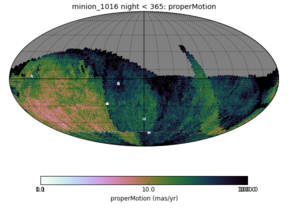
\includegraphics[width=2.0in]{./figs/milkyway/astromPanels/MW_Astrom_pmError_Baseline_01y_map.png}
  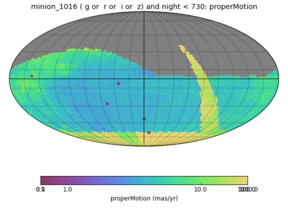
\includegraphics[width=2.0in]{./figs/milkyway/astromPanels/MW_Astrom_pmError_Baseline_02y_map.png}
  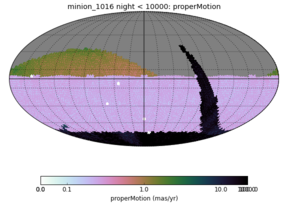
\includegraphics[width=2.0in]{./figs/milkyway/astromPanels/MW_Astrom_pmError_Baseline_10y_map.png}
  \end{center}
  \begin{center}
  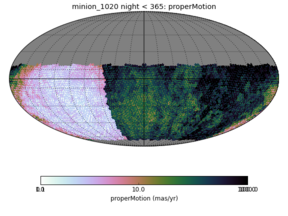
\includegraphics[width=2.0in]{./figs/milkyway/astromPanels/MW_Astrom_pmError_PanSTARRS_01y_map.png}
  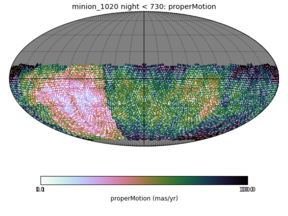
\includegraphics[width=2.0in]{./figs/milkyway/astromPanels/MW_Astrom_pmError_PanSTARRS_02y_map.png}
  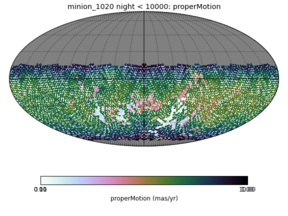
\includegraphics[width=2.0in]{./figs/milkyway/astromPanels/MW_Astrom_pmError_PanSTARRS_10y_map.png}
  \end{center}

  \begin{center}
  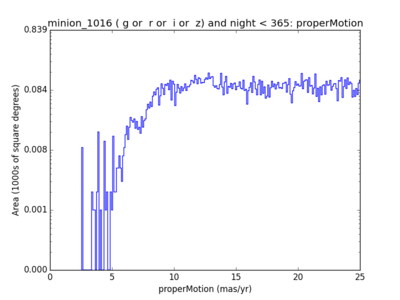
\includegraphics[width=2.0in]{./figs/milkyway/astromPanels/MW_Astrom_pmError_Baseline_01y_hst.png}
  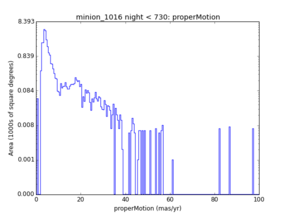
\includegraphics[width=2.0in]{./figs/milkyway/astromPanels/MW_Astrom_pmError_Baseline_02y_hst.png}
  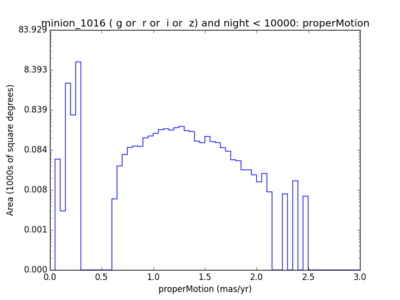
\includegraphics[width=2.0in]{./figs/milkyway/astromPanels/MW_Astrom_pmError_Baseline_10y_hst.png}
  \end{center}
  \begin{center}
  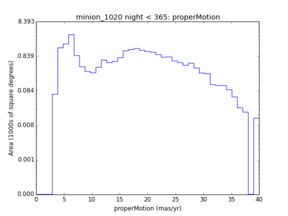
\includegraphics[width=2.0in]{./figs/milkyway/astromPanels/MW_Astrom_pmError_PanSTARRS_01y_hst.png}
  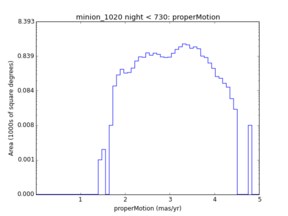
\includegraphics[width=2.0in]{./figs/milkyway/astromPanels/MW_Astrom_pmError_PanSTARRS_02y_hst.png}
  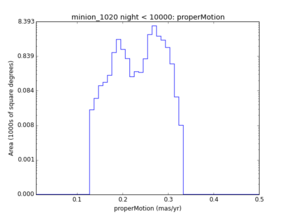
\includegraphics[width=2.0in]{./figs/milkyway/astromPanels/MW_Astrom_pmError_PanSTARRS_10y_hst.png}
  \end{center}
  \caption{Proper motion error for a star at $r=21.0$, for different epochs within the survey. Crowding errors are ignored. {\it Top and Third row:} OpSim run \opsimdbref{db:baseCadence}. {\it Second and bottom row:} OpSim run \opsimdbref{db:opstwoPS} (PanSTARRS-like cadence). Reading left-right, columns represent: {\it Left column:} all observations within the first 365 days of operation; {\it Middle column:} first two years; {\it right column:} the full 10-year survey. Spatial maps are clipped at 95\% and a log-scale is used for the maps and histograms. NOTE: the horizontal axes in the histograms are different for the two strategies; this is to allow the long tail of the proper motion error distribution in the \opsimdbref{db:baseCadence} to be displayed.}
  \label{fig_astrom_ByTime_pmError}
\end{figure}


\begin{figure}[ht]
  \begin{center}
  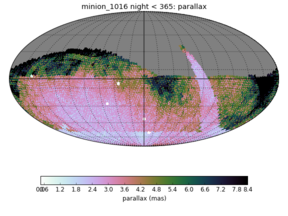
\includegraphics[width=2.0in]{./figs/milkyway/astromPanels/MW_Astrom_paError_Baseline_01y_map.png}
  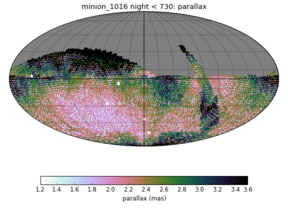
\includegraphics[width=2.0in]{./figs/milkyway/astromPanels/MW_Astrom_paError_Baseline_02y_map.png}
  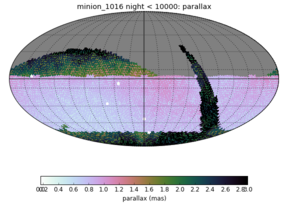
\includegraphics[width=2.0in]{./figs/milkyway/astromPanels/MW_Astrom_paError_Baseline_10y_map.png}
  \end{center}
  \begin{center}
  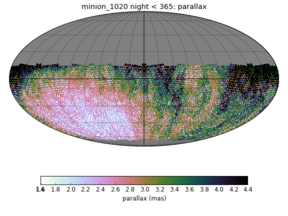
\includegraphics[width=2.0in]{./figs/milkyway/astromPanels/MW_Astrom_paError_PanSTARRS_01y_map.png}
  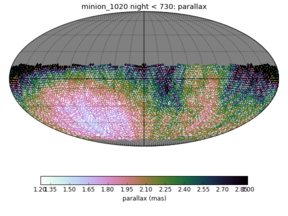
\includegraphics[width=2.0in]{./figs/milkyway/astromPanels/MW_Astrom_paError_PanSTARRS_02y_map.png}
  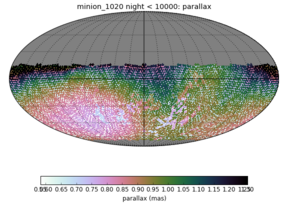
\includegraphics[width=2.0in]{./figs/milkyway/astromPanels/MW_Astrom_paError_PanSTARRS_10y_map.png}
  \end{center}

  \begin{center}
  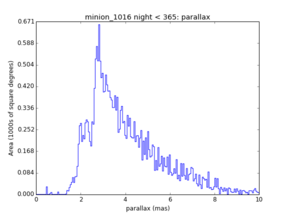
\includegraphics[width=2.0in]{./figs/milkyway/astromPanels/MW_Astrom_paError_Baseline_01y_hst.png}
  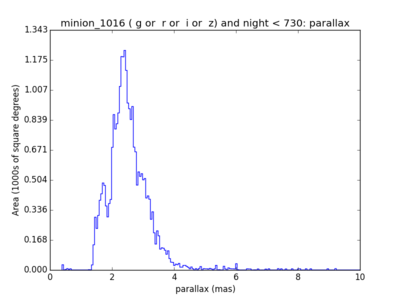
\includegraphics[width=2.0in]{./figs/milkyway/astromPanels/MW_Astrom_paError_Baseline_02y_hst.png}
  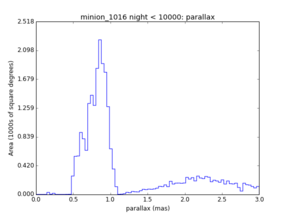
\includegraphics[width=2.0in]{./figs/milkyway/astromPanels/MW_Astrom_paError_Baseline_10y_hst.png}
  \end{center}
  \begin{center}
  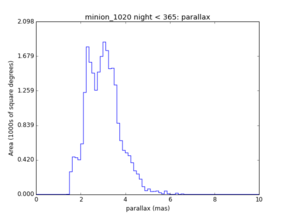
\includegraphics[width=2.0in]{./figs/milkyway/astromPanels/MW_Astrom_paError_PanSTARRS_01y_hst.png}
  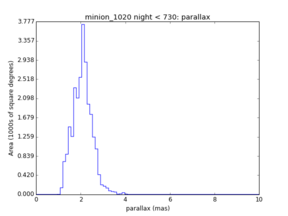
\includegraphics[width=2.0in]{./figs/milkyway/astromPanels/MW_Astrom_paError_PanSTARRS_02y_hst.png}
  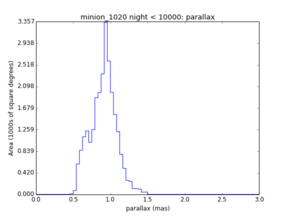
\includegraphics[width=2.0in]{./figs/milkyway/astromPanels/MW_Astrom_paError_PanSTARRS_10y_hst.png}
  \end{center}
  \caption{Parallax error for a star at $r=21.0$, for different epochs within the survey. Crowding errors are ignored. {\it Top and Third row:} OpSim run \opsimdbref{db:baseCadence}. {\it Second and bottom row:} OpSim run \opsimdbref{db:opstwoPS} (PanSTARRS-like cadence). Reading left-right, columns represent: {\it Left column:} all observations within the first 365 days of operation; {\it Middle column:} first two years; {\it right column:} the full 10-year survey. Spatial maps are clipped at 95\%.}
  \label{fig_astrom_ByTime_paError}
\end{figure}

%%% Now for the metrics by filter.
\begin{figure}[ht]
  \begin{center}
  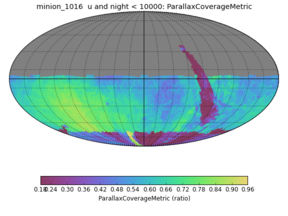
\includegraphics[width=2.0in]{./figs/milkyway/astromPanels/MW_Astrom_paCovge_Baseline_u_map.png}
  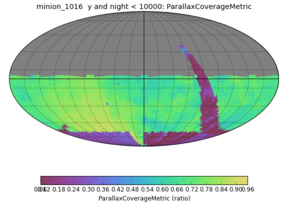
\includegraphics[width=2.0in]{./figs/milkyway/astromPanels/MW_Astrom_paCovge_Baseline_y_map.png}
  \includegraphics[width=2.0in]{./figs/milkyway/astromPanels/MW_Astrom_paCovge_Baseline_10y_map.png}
  \end{center}
  \begin{center}
  \includegraphics[width=2.0in]{./figs/milkyway/astromPanels/MW_Astrom_paCovge_PanSTARRS_u_map.png}
  \includegraphics[width=2.0in]{./figs/milkyway/astromPanels/MW_Astrom_paCovge_PanSTARRS_y_map.png}
  \includegraphics[width=2.0in]{./figs/milkyway/astromPanels/MW_Astrom_paCovge_PanSTARRS_10y_map.png}
  \end{center}

  \begin{center}
  \includegraphics[width=2.0in]{./figs/milkyway/astromPanels/MW_Astrom_paCovge_Baseline_u_hst.png}
  \includegraphics[width=2.0in]{./figs/milkyway/astromPanels/MW_Astrom_paCovge_Baseline_y_hst.png}
  \includegraphics[width=2.0in]{./figs/milkyway/astromPanels/MW_Astrom_paCovge_Baseline_10y_hst.png}
  \end{center}
  \begin{center}
  \includegraphics[width=2.0in]{./figs/milkyway/astromPanels/MW_Astrom_paCovge_PanSTARRS_u_hst.png}
  \includegraphics[width=2.0in]{./figs/milkyway/astromPanels/MW_Astrom_paCovge_PanSTARRS_y_hst.png}
  \includegraphics[width=2.0in]{./figs/milkyway/astromPanels/MW_Astrom_paCovge_PanSTARRS_10y_hst.png}
  \end{center}
  \caption{Parallax coverage achieved for three extremes of object color, over the full 10-year survey. {\it Top and Third row:} OpSim run \opsimdbref{db:baseCadence}. {\it Second and bottom row:} OpSim run \opsimdbref{db:opstwoPS} (PanSTARRS-like cadence). Reading left-right, columns represent: {\it Left column:} Objects detected only in the bluest filter; {\it Middle column:} objects detected only in the reddest filter; {\it Right column:} objects detected in all filters. Spatial maps are clipped at 95\%, with histogram horizontal scale set to $\pm 1.0$~for easy comparison.}
  \label{fig_astrom_ByFilter_PACoverage}
\end{figure}

\begin{figure}[ht]
  \begin{center}
  \includegraphics[width=2.0in]{./figs/milkyway/astromPanels/MW_Astrom_paDegen_Baseline_u_map.png}
  \includegraphics[width=2.0in]{./figs/milkyway/astromPanels/MW_Astrom_paDegen_Baseline_y_map.png}
  \includegraphics[width=2.0in]{./figs/milkyway/astromPanels/MW_Astrom_paDegen_Baseline_10y_map.png}
  \end{center}
  \begin{center}
  \includegraphics[width=2.0in]{./figs/milkyway/astromPanels/MW_Astrom_paDegen_PanSTARRS_u_map.png}
  \includegraphics[width=2.0in]{./figs/milkyway/astromPanels/MW_Astrom_paDegen_PanSTARRS_y_map.png}
  \includegraphics[width=2.0in]{./figs/milkyway/astromPanels/MW_Astrom_paDegen_PanSTARRS_10y_map.png}
  \end{center}

  \begin{center}
  \includegraphics[width=2.0in]{./figs/milkyway/astromPanels/MW_Astrom_paDegen_Baseline_u_hst.png}
  \includegraphics[width=2.0in]{./figs/milkyway/astromPanels/MW_Astrom_paDegen_Baseline_y_hst.png}
  \includegraphics[width=2.0in]{./figs/milkyway/astromPanels/MW_Astrom_paDegen_Baseline_10y_hst.png}
  \end{center}
  \begin{center}
  \includegraphics[width=2.0in]{./figs/milkyway/astromPanels/MW_Astrom_paDegen_PanSTARRS_u_hst.png}
  \includegraphics[width=2.0in]{./figs/milkyway/astromPanels/MW_Astrom_paDegen_PanSTARRS_y_hst.png}
  \includegraphics[width=2.0in]{./figs/milkyway/astromPanels/MW_Astrom_paDegen_PanSTARRS_10y_hst.png}
  \end{center}
  \caption{Parallax degeneracy with hour angle, selecting filters for three extremes of object color, over the full 10-year survey. {\it Top and Third row:} OpSim run \opsimdbref{db:baseCadence}. {\it Second and bottom row:} OpSim run \opsimdbref{db:opstwoPS} (PanSTARRS-like cadence). Reading left-right, columns represent: {\it Left column:} Objects detected only in the bluest filter; {\it Middle column:} objects detected only in the reddest filter; {\it Right column:} objects detected in all filters. Spatial maps are clipped at 95\%, with histogram horizontal scale set to the range $0.0-1.0$.}
  \label{fig_astrom_ByFilter_PADegen}
\end{figure}

\begin{figure}[ht]
  \begin{center}
  \includegraphics[width=2.0in]{./figs/milkyway/astromPanels/MW_Astrom_pmError_Baseline_u_map.png}
  \includegraphics[width=2.0in]{./figs/milkyway/astromPanels/MW_Astrom_pmError_Baseline_y_map.png}
  \includegraphics[width=2.0in]{./figs/milkyway/astromPanels/MW_Astrom_pmError_Baseline_10y_map.png}
  \end{center}
  \begin{center}
  \includegraphics[width=2.0in]{./figs/milkyway/astromPanels/MW_Astrom_pmError_PanSTARRS_u_map.png}
  \includegraphics[width=2.0in]{./figs/milkyway/astromPanels/MW_Astrom_pmError_PanSTARRS_y_map.png}
  \includegraphics[width=2.0in]{./figs/milkyway/astromPanels/MW_Astrom_pmError_PanSTARRS_10y_map.png}
  \end{center}

  \begin{center}
  \includegraphics[width=2.0in]{./figs/milkyway/astromPanels/MW_Astrom_pmError_Baseline_u_hst.png}
  \includegraphics[width=2.0in]{./figs/milkyway/astromPanels/MW_Astrom_pmError_Baseline_y_hst.png}
  \includegraphics[width=2.0in]{./figs/milkyway/astromPanels/MW_Astrom_pmError_Baseline_10y_hst.png}
  \end{center}
  \begin{center}
  \includegraphics[width=2.0in]{./figs/milkyway/astromPanels/MW_Astrom_pmError_PanSTARRS_u_hst.png}
  \includegraphics[width=2.0in]{./figs/milkyway/astromPanels/MW_Astrom_pmError_PanSTARRS_y_hst.png}
  \includegraphics[width=2.0in]{./figs/milkyway/astromPanels/MW_Astrom_pmError_PanSTARRS_10y_hst.png}
  \end{center}
  \caption{Proper motion error for a star at apparent magnitude $m=21.0$, for three extremes of object color and assessed over the full survey. Crowding errors are ignored. {\it Top and Third row:} OpSim run \opsimdbref{db:baseCadence}. {\it Second and bottom row:} OpSim run \opsimdbref{db:opstwoPS} (PanSTARRS-like cadence). Reading left-right, columns represent: {\it Left column:} Objects detected only in the bluest filter; the fiducial object has apparent magnitude $u=21.0$; {\it Middle column:} objects detected only in the reddest filter (so $y = 21.0$); {\it Right column:} objects detected in all filters (using $r=21.0$~and a ``flat'' spectrum within sims\_maf). Spatial maps are clipped at 95\% and a log-scale is used for both the spatial maps and histograms. NOTE: the horizontal axes in the histograms are different for the two strategies; this is to allow the long tail of the proper motion error distribution in the \opsimdbref{db:baseCadence} to be displayed. \new{Horizontal scales on histograms may need adjusting.}}
  \label{fig_astrom_ByFilter_pmError}
\end{figure}

\begin{figure}[ht]
  \begin{center}
  \includegraphics[width=2.0in]{./figs/milkyway/astromPanels/MW_Astrom_paError_Baseline_u_map.png}
  \includegraphics[width=2.0in]{./figs/milkyway/astromPanels/MW_Astrom_paError_Baseline_y_map.png}
  \includegraphics[width=2.0in]{./figs/milkyway/astromPanels/MW_Astrom_paError_Baseline_10y_map.png}
  \end{center}
  \begin{center}
  \includegraphics[width=2.0in]{./figs/milkyway/astromPanels/MW_Astrom_paError_PanSTARRS_u_map.png}
  \includegraphics[width=2.0in]{./figs/milkyway/astromPanels/MW_Astrom_paError_PanSTARRS_y_map.png}
  \includegraphics[width=2.0in]{./figs/milkyway/astromPanels/MW_Astrom_paError_PanSTARRS_10y_map.png}
  \end{center}

  \begin{center}
  \includegraphics[width=2.0in]{./figs/milkyway/astromPanels/MW_Astrom_paError_Baseline_u_hst.png}
  \includegraphics[width=2.0in]{./figs/milkyway/astromPanels/MW_Astrom_paError_Baseline_y_hst.png}
  \includegraphics[width=2.0in]{./figs/milkyway/astromPanels/MW_Astrom_paError_Baseline_10y_hst.png}
  \end{center}
  \begin{center}
  \includegraphics[width=2.0in]{./figs/milkyway/astromPanels/MW_Astrom_paError_PanSTARRS_u_hst.png}
  \includegraphics[width=2.0in]{./figs/milkyway/astromPanels/MW_Astrom_paError_PanSTARRS_y_hst.png}
  \includegraphics[width=2.0in]{./figs/milkyway/astromPanels/MW_Astrom_paError_PanSTARRS_10y_hst.png}
  \end{center}
  \caption{Parallax error for a star at apparent magnitude $m=21.0$, for three extremes of object color and assessed over the full survey. Crowding errors are ignored. {\it Top and Third row:} OpSim run \opsimdbref{db:baseCadence}. {\it Second and bottom row:} OpSim run \opsimdbref{db:opstwoPS} (PanSTARRS-like cadence). Reading left-right, columns represent: {\it Left column:} Objects detected only in the bluest filter; the fiducial object has apparent magnitude $u=21.0$; {\it Middle column:} objects detected only in the reddest filter (so $y = 21.0$); {\it Right column:} objects detected in all filters (using $r=21.0$~and a ``flat'' spectrum within sims\_maf). Spatial maps are clipped at 95\%.}
  \label{fig_astrom_ByFilter_paError}
\end{figure}

\subsubsection{Figures of Merit depening on the Metrics}

Building on the first-order metrics above, this subsection will communicate scientific figures of merit for the cases identified in \autoref{sec:\secname:MW_Astrometry_measurements} above.

\new{Table \ref{tab_SummaryMWAstrometry} summarizes the Figures of Merit for Astrometry science cases.}

\subsection{Topics that will need to be addressed}
\label{sec:\secname:MW_Astrometry_furtherwork}

Here we present suggestions for further work, first on figures of
merit for the science cases, and then on additional Metrics for LSST's
astrometric performance.

\subsubsection{Further work on science Figures of Merit}
%\medskip

As of 2016-01-04, the Figures of Merit for both the highlighted
Science cases need to be implemented and applied to OpSim output,
preferably in a format that can be summarized in a single Table in
this section. These figures of merit are discussed above in Section
\ref{sec:\secname:MW_Astrometry_metrics} (particularly for the Halo
Streams science project). Figures of merit for the two science cases
might be:
\begin{itemize}
  \item[1.] Number of streams that LSST can discover via their proper motions;
\item[2.] Uncertainty and bias in the thin and thick disk differential age measurement when using white dwarfs from each population as tracers.
\end{itemize}

Given the diversity of science cases that use local Solar Neighborhood
populations as tracers, it may be advantageous to subdivide the Solar
Neighborhood projects into further figures of merit. Two further example
figures of merit might then be:
\begin{itemize}
  \item[3.] Uncertainty and bias in the Brown Dwarf mass function using Solar Neighborhood tracers;
   \item[4.] Uncertainty and bias in the thickness in the main sequence of M-dwarfs within 25pc from the Sun, once variability has been characterized and removed.
\end{itemize}

%%%% SUMMARY TABLE FOR THIS SECTION

\begin{table}
  \begin{tabular}{l|p{6cm}|c|c|c|c|p{5cm}}
    FoM & Brief description & {\rotatebox{90}{\opsimdbref{db:baseCadence} }} & {\rotatebox{90}{\opsimdbref{db:opstwoPS} }} & {\rotatebox{90}{\scriptsize{\tt astro\_lsst\_01\_1004} }} &  {\rotatebox{90}{future run 2}} & Notes \\
    \hline
    1.1 & \footnotesize{Median parallax error at $g=21$ (main survey)}      & - & - & - & - & \footnotesize{Summarize the presentation in Figures \ref{fig_astrom_ByTime_PACoverage}-\ref{fig_astrom_ByFilter_paError}} \\
    1.2. & \footnotesize{Median parallax error at $g=21$ (plane)}   & - & - & - & - &  - \\
    1.3. & \footnotesize{Median proper motion error at $g=21$ (main survey)}  & - & - & - & - &  \footnotesize{Take median of Figure \ref{fig_astrom_ByTime_pmError} over the ``plane'' region.~~~ \new{2016-04-26 Note to Phil when Section-auditing: I (WIC) still intend to evaluate this before the Apr 30th deadline! Peter Y has suggested a way this might be done.}  } \\
    1.4. & \footnotesize{Median proper motion error at $g=21$ (plane)} & - & - & - & - &  - \\
    \hline
    2.1. & \footnotesize{Number of streams LSST can discover via proper motions} & - & - & - & - &  - \\
    3.1. & \footnotesize{Uncertainty and bias in thin- and thick-disk differential age measurement via white dwarfs} & - & - & - & - &  - \\
    4.1. & \footnotesize{Uncertainty and bias in brown dwarf mass function from the Solar Neighborhood}  & - & - & - & - & \footnotesize{Using astrometry metrics for objects detected only in the reddest filter(s)} \\
    4.2. & \footnotesize{Uncertainty and bias in white dwarf mass function from the Solar Neighborhood}  & - & - & - & - & \footnotesize{Using astrometry metrics for objects detected only in the bluest filter(s)} \\
    5.1. & \footnotesize{Uncertainty and bias in Solar Neighborhood M-dwarf thickness on the MS}  & - & - & - & - &  - \\
\end{tabular}
\caption{Summary of Figures of Merit for the Milky Way Astrometry science cases. The best value of each FoM is indicated in bold. Runs \opsimdbref{db:baseCadence} and \opsimdbref{db:opstwoPS} refer to the Baseline and PanSTARRS-like strategies, respectively. Column {\tt astro\_lsst\_01\_1004} refers to a recently-completed OpSim run that includes the Plane in Wide-Fast-Deep observations. See \autoref{sec:MW_Astrometry}.}
\label{tab_SummaryMWAstrometry}
\end{table}


%%%% SUMMARY TABLE FINISHES HERE


\subsubsection{Further work on Astrometry Metrics}

The MAF metrics presented in Sections \ref{sec:\secname:MW_Astrometry_OpSim} and \ref{sec:\secname:MW_Astrometry_metrics} are only part of the
study of LSST's predicted astrometric performance.  Detailed simulations
and studies need to be done in many other areas as part of the
prediction and verification of LSST's astrometric performance.  Among
the most important are the following.
\begin{itemize}
\item How well do galaxies perform as astrometric reference objects? Are certain shapes or colors better than others? What is the
surface density of ``good" astrometric reference galaxies as a function of filter?
\item How well can we identify optically point-like QSOs that will be useful in matching the optical reference frame to the ICRS?
%\item Given the LSST exposure time, site, and physical characteristics, how can we mitigate the limitations on astrometric accuracy imposed by the seeing and local atmospheric turbulence?
\item How does the astrometric performance depend on stellar density? If there are fields in which photometry is only possible via difference imaging, what are the limitations
on astrometry in these fields?
%\item What tools do we need to compare the general and specific agreement between the {\it Gaia} results and the LSST results?
\item Does the ``brighter-wider" effect in the deep-depletion CCDs introduce a magnitude term into the centroid positions?
\end{itemize}

\navigationbar

% --------------------------------------------------------------------
